\documentclass[11pt,a4paper]{article}
\usepackage[margin=1in]{geometry}
\usepackage{float}
\usepackage{graphicx}
\usepackage{amsmath}
\usepackage{enumitem}
\usepackage{hyperref}
\hypersetup{colorlinks=true,linkcolor=blue,urlcolor=blue}
\title{COL334 Assignment 2 Report}
\author{Samyak Sanghvi (2023CS10807) \\ Namit Jain (2023CS10483)}
% \date{September 2025}
\begin{document}
\maketitle
% \tableofcontents
% \newpage

\section{Part 1: Word Counting over TCP}
\subsection{Goal}
Implement a basic TCP client and server that transfer a list of comma--separated words in fixed--sized batches using a simple request--response protocol, and study how batching size $k$ affects total completion time.

\subsection{Protocol Summary}
The client incrementally downloads the word list by repeatedly asking for $k$ words starting at an offset $p$. The server responds with up to $k$ words and appends an ``EOF'' token when the end of file is reached.

\subsection{Server Workflow}
\begin{enumerate}[leftmargin=1.2cm]
  \item Read configuration (IP, port, default $k$, starting offset $p$, word file name, repetitions).
  \item Load the entire word list (single comma--separated line) into an in\-memory vector.
  \item Create a TCP socket, bind to configured port, listen.
  \item For each accepted connection, loop reading one line requests of the form ``offset,k''.
  \item For each request: slice the word vector, build a comma\-separated response, append ``EOF'' if the end is reached, send line. If offset already beyond end, reply ``EOF" immediately.
  \item Close connection when client stops sending or EOF delivered.
\end{enumerate}

\subsection{Client Workflow}
\begin{enumerate}[leftmargin=1.2cm]
  \item Read configuration; optionally override $k$ via command line.
  \item For each iteration (repeat count): open a TCP connection to the server.
  \item Initialize offset $= p$. While not finished:
    \begin{enumerate}
      \item Send line ``offset,k''. \item Receive one response line. \item If it is exactly ``EOF'' stop. \item Otherwise tokenise words, count frequencies, detect the presence of trailing ``EOF" token; if not present increment offset by $k$ and continue.
    \end{enumerate}
  \item After finishing all iterations, output word frequency counts and total elapsed milliseconds.
\end{enumerate}

\subsection{Experiment Design}
We varied $k$ over a predefined set (e.g., $\{1,2,5,10,20,50,100\}$). For each value, we ran the full download five times and recorded total completion time. The harness stored raw timings in a CSV, then a plotting script computed mean and (normal approximation) 95\% confidence intervals.

\subsection{Observations}
\textbf{Trend:} Increasing $k$ substantially reduces completion time initially because per\-request fixed costs (TCP send/recv syscalls, user\-kernel crossings, framing) are amortized across more payload data. Beyond a certain $k$, the curve flattens: residual time is dominated by total bytes transferred plus constant connection setup overhead per iteration. Extremely large $k$ would not reduce time further because the entire file already fits in a small number of batches. Empirically the marginal improvement between the largest two $k$ values was negligible, indicating a knee point. Confidence intervals narrowed for larger $k$ due to fewer round trips and less variance from scheduling jitter.

\subsection{Result Plot}
Figure~\ref{fig:p1} shows the mean completion time vs $k$.

\begin{figure}[H]
  \centering
  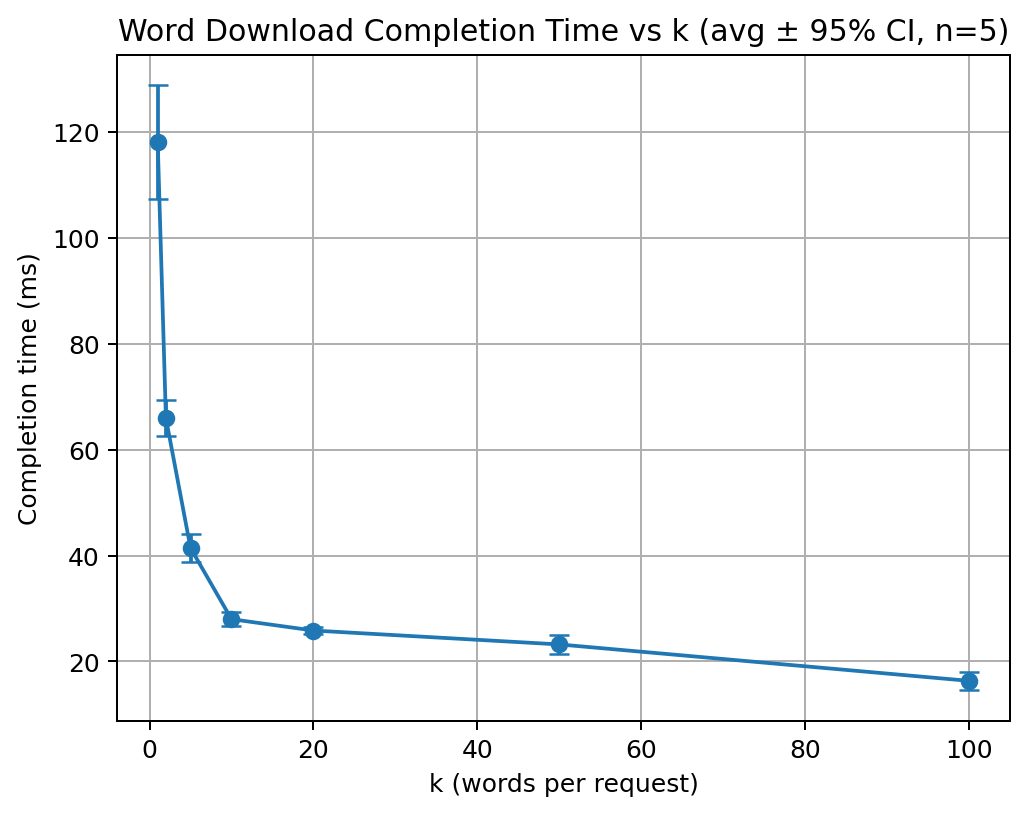
\includegraphics[width=0.7\linewidth]{part1/p1_plot.png}
  \caption{Part 1: Completion time (ms) vs batch size $k$ with 95\% CI.}
  \label{fig:p1}
\end{figure}

\section{Part 2: Concurrent Clients (Serialized Service)}
\subsection{Goal}
Extend the system to multiple concurrent clients connecting to the same server port. The server accepts many simultaneous TCP connections but serves requests \emph{one at a time} (FCFS) by queueing connections, thereby exposing the impact of contention.

\subsection{Server Architecture}
Two threads were used for clarity:
\begin{enumerate}[leftmargin=1.2cm]
  \item \textbf{Listener Thread:} Accepts incoming connections rapidly and enqueues them.
  \item \textbf{Worker Thread:} Dequeues one connection at a time and processes its request sequence to completion (until EOF for that client), then moves to the next connection.
\end{enumerate}
This models FCFS at the granularity of a whole file download.

\subsection{Client Behavior}
Each client independently performs the same batch download logic as Part~1. All clients start near-simultaneously, causing a queue to build when more than one client is active.

\subsection{Experiment Design}
We varied the number of concurrent clients in $\{1,5,9,13,17,21,25,29,32\}$ (step 4 up to 32). For each level we ran five trials. For every client we extracted its completion time; we then computed the mean per\-client completion time for that trial (i.e., average over the $n$ clients), and aggregated these means across repeats to derive overall mean and 95\% confidence intervals for each concurrency level.

\subsection{Observations}
\textbf{Scaling Effect:} Average completion time per client increased approximately linearly once the queue became non\-empty because only one entire download is serviced at a time; added clients predominantly wait. \textbf{Diminishing Throughput:} Aggregate throughput (clients finished per unit wall time) remains roughly constant after the initial increase since the server is fully utilized. \textbf{Variance:} Confidence intervals widen with more clients due to timing jitter accumulation and slight differences in start ordering.

\subsection{Result Plot}
Figure~\ref{fig:p2} illustrates the rise in average per\-client completion time with concurrency.

\begin{figure}[H]
  \centering
  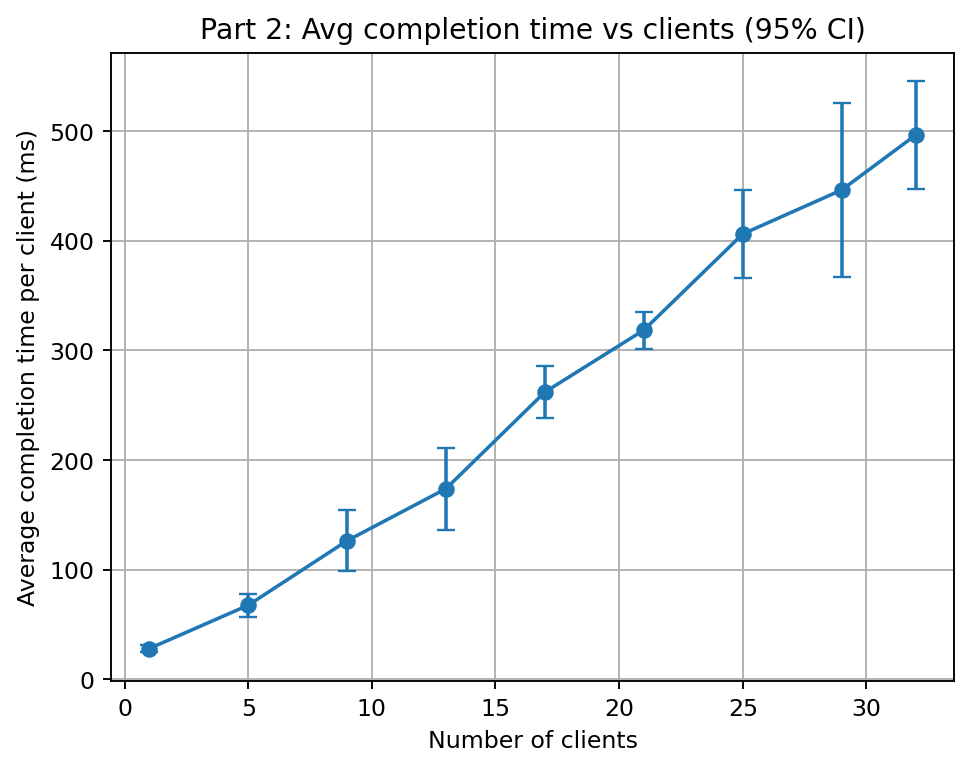
\includegraphics[width=0.7\linewidth]{part2/p2_plot.png}
  \caption{Part 2: Average completion time per client vs number of clients (95\% CI).}
  \label{fig:p2}
\end{figure}

\section{Part 3: Greedy Client under FCFS}
\subsection{Goal}
Investigate fairness when one client behaves greedily by issuing $c$ back-to-back download attempts, while the server processes clients in strict FCFS order (one whole download per client before moving to the next).

\subsection{Setup}
Ten clients participate: one greedy, nine normal. Each uses a fixed request packet size $k=5$ words. The greedy client sends $c$ requests without waiting for a response (back-to-back) and then after receiving all responses, it sends next batch of $c$ requests. Whereas, the normal clients are sending one request and waiting for the response, and only then are they sending the next request.

\subsection{Metric (what $x_i$ means)}
Fairness is quantified with Jain's Fairness Index (JFI)
\[
\mathrm{JFI} \;=\; \frac{\left(\sum_{i=1}^n x_i\right)^2}{n \cdot \sum_{i=1}^n x_i^2},
\]
where here \emph{$x_i$ is the reciprocal of client $i$'s completion time} (i.e., higher $x_i$ means the client finished sooner). This is scale-invariant and directly rewards faster completion.

\subsection{Experiment}
We varied $c \in \{1,\dots,20\}$. For each $c$, we measured all clients' completion times $T_i$, set $x_i = 1/T_i$, and computed JFI (optionally averaged across repeats).

\subsection{Observations}
\textbf{Baseline ($c=1$).} All clients get comparable service; JFI is close to~1.\\
\textbf{As $c$ increases.} Because FCFS serves one whole download at a time, the greedy client repeatedly occupies the server while others wait, so the spread in $\{x_i\}$ grows and JFI falls. In practice the drop is sharp at small $c$ and then tapers as we continue to increase the value of $c$. \\
We also notice that the plots of $JFI$ vs $c$ and $completion$ $time$ vs $c$ are highly correlated. 

\subsection{What value can the JFI value can go down to? (\(c \rightarrow \infty\))}
Suppose with $c=1$ the fair per-client completion time is about $4000$\,ms. If $c$ is very large, the greedy client effectively completes as if it were alone, so its time approaches $\approx 4000/10=400$\,ms, while the others are each still around $\approx 4000$\,ms. This is because, in the worst case scenario for large $c$, greedy client will complete all its requests while among others, the most number of requests processed will be $1$. Hence, using $x_g=1/400$ and $x_o=1/4000$,
\[
\sum x_i = x_g + 9x_o = \frac{1}{400}+\frac{9}{4000} = \frac{19}{4000},\qquad
\sum x_i^2 = \frac{1}{400^2} + 9\cdot \frac{1}{4000^2} = \frac{100+9}{4000^2} = \frac{109}{4000^2}.
\]
Hence
\[
\mathrm{JFI} \;=\; \frac{\left(\frac{19}{4000}\right)^2}{10 \cdot \frac{109}{4000^2}}
\;=\; \frac{19^2}{10 \cdot 109}
\;=\; \frac{361}{1090}
\;\approx\; 0.331.
\]
This rough calculation matches the empirical lower end we observe for large $c$.

\subsection{Result Plots}
\begin{figure}[H]
  \centering
  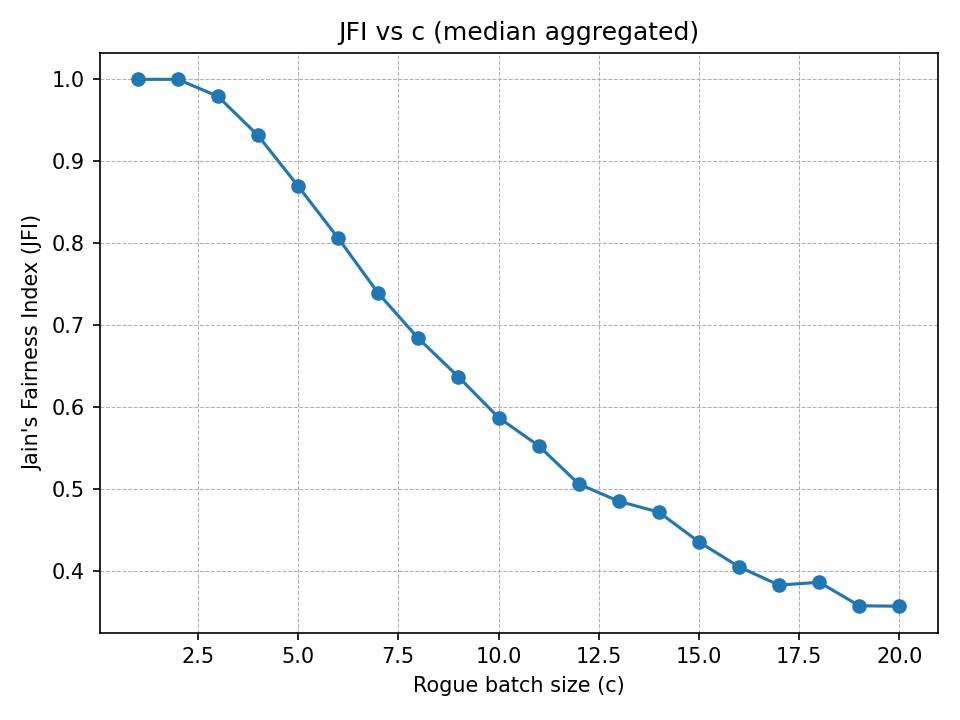
\includegraphics[width=0.6\linewidth]{part3/plot_JFI.png}
  \caption{JFI vs greedy burst size $c$ using $x_i=1/T_i$.}
  \label{fig:p3_jfi}
\end{figure}

\begin{figure}[H]
  \centering
  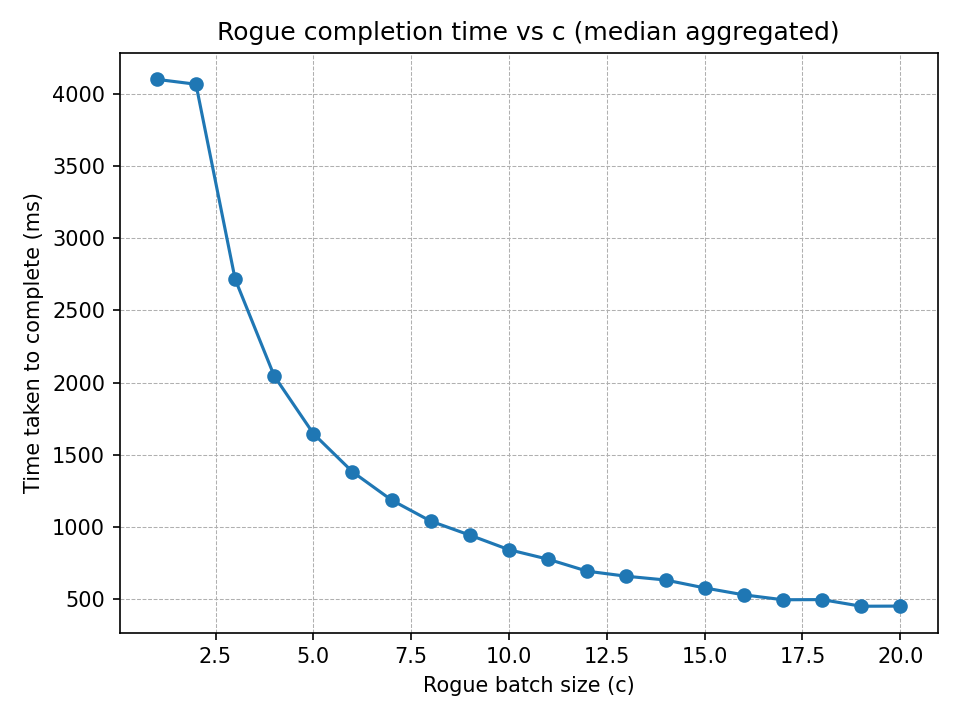
\includegraphics[width=0.6\linewidth]{part3/plot_T.png}
  \caption{Greedy client's completion time vs $c$.}
  \label{fig:p3_T}
\end{figure}

\subsection{Code sketch (what runs where)}
\\

\textbf{Server (FCFS mode):} One thread accepts and enqueues connections; a worker thread services them strictly in arrival order, running a full request sequence to EOF for a client before moving on. For more stable results, the config file also contains: \\
1) $trials$ : will run the simulation these number of times. And then take the median of all the results received with respect to each client for a particular $c$. \\
2) $repeat$ : will copy the entire content of the $word.txt$ file over these many times. \\
\textbf{Clients:} We launch 10 clients nearly simultaneously. The greedy client runs $c$ complete downloads back-to-back; the other 9 run one each. Each client logs, its requests sent, responses received and its total completion time. The analysis script converts times to $x_i=1/T_i$ and computes JFI.

\section{Part 4: Round Robin Scheduling}
\subsection{Goal}
Replace FCFS with a policy that prevents one client from getting consecutive responses while others are waiting. We use a simple round-robin loop that, at each step, serves \emph{at most one response} for the current client and then moves to the next active client.

\subsection{Server Workflow (RR mode)}
Maintain a list of active connections. Iterate over it cyclically; when a client has a pending request, send one response, and move to the next client. An $idx$ variable is increased and moded by $n\textunderscore clients$ (number of clients) at every iteration. And remove a client after it receives an EOF response.

\subsection{Experiment}
Same setup as Part 3 ($n=10$, one greedy client, $c=1..10$, $k=5$). We measure completion times, set $x_i=1/T_i$, and compute JFI for each $c$.

\subsection{Observations}
\textbf{Fairness stays high.} Because no client can receive two consecutive responses while others are pending, the per-client throughputs $\{x_i\}$ remain close, so JFI stays near~1 for all $c$.

\subsection{Why RR pushes JFI $\approx 1$ (intuitive)}
Round-robin alternation prevents any client from hogging the server: once a client gets a response, the server immediately switches to others that are ready. With identical request sizes ($k$ is fixed) and the same network path, each client receives comparable attention over time. With respect to each client, the server will store a buffer of pending requests but it won't act upon it. A client will only get its next response when one entire loop of responses across all clients have been completed, so no matter how many the number of pending requests are wrt each client, the server will give fair chance to every client to receive response. As a result their reciprocals of completion time, $x_i=1/T_i$, cluster tightly, which mathematically drives JFI very close to~1.

\subsection{Result Plots}
\begin{figure}[H]
  \centering
  
\includegraphics[width=0.6\linewidth]{part4/plot_JFI.png}
  \caption{Part 4 (RR): JFI vs $c$ using $x_i=1/T_i$.}
  \label{fig:p4_jfi}
\end{figure}

\begin{figure}[H]
  \centering
  
\includegraphics[width=0.6\linewidth]{part4/plot_T.png}
  \caption{Part 4 (RR): Greedy client's completion time vs $c$.}
  \label{fig:p4_T}
\end{figure}

\\


\textbf{Why JFI is close to, but not exactly, 1.} Consecutive responses can take slightly different wall-clock times due to OS scheduling, socket buffer effects, and minor request/response size differences near the end of a file. Clients also do not start at the exact same instant, so some experience a tiny head-start or head-lag. With all clients running concurrently, these small timing asymmetries introduce unavoidable noise, which shows up as a tiny deviation from $1$.
\\

\textbf{Drawback.} Unweighted round robin gives every active client equal turns regardless of remaining work or urgency. When some clients need far fewer responses or have tighter deadlines, this interleaving can inflate their completion time; a weighted or priority policy would better match heterogeneous needs. It worked well in this scenario because the requirement of each client was identical.

\subsection{Code sketch (RR path)}
\textbf{Server (RR mode):} A listener accepts sockets and registers each in an \texttt{active} list. A scheduler loop walks this list in order and services at most one pending request per client per pass. Shared state (e.g., per-socket pending queues) is protected with a lock and condition variable.\\
\textbf{Clients and analysis:} Same as Part 3; we only switch \texttt{mode} to \texttt{rr}. We compute $x_i=1/T_i$ and then JFI.

\section*{Key Takeaways}
\begin{itemize}
  \item Batching (larger $k$) reduces per\-request overhead until dominated by bulk transfer cost.
  \item Serialized whole\-download FCFS scales poorly in per\-client latency as concurrency rises.
  \item Greedy behavior exploits FCFS by occupying consecutive service slots, sharply reducing fairness (lower JFI).
  \item Round Robin restores fairness by enforcing temporal sharing, keeping JFI high across greediness levels.
  \item Scheduling granularity and consistent request sizes are crucial for robust fairness guarantees.
\end{itemize}

\end{document}